% This will be the main document for the Technical Networks paper to
% be written by the Eggnet team of Jordan Ell, Triet Huynh and Braden
% Simpson in association with Adrian Schroeter and Daniela Damian.

\documentclass[conference]{IEEEtran}

% Use of outside images
\usepackage{graphicx} 
% Use text inside euqations
\usepackage{amsmath}

% Correct bad hyphenation here
\hyphenation{op-tical net-works semi-conduc-tor}

% Begin the paper here
\begin{document}


% Paper title
% Can use linebreaks \\ within to get better formatting as desired
\title{Finding Harmful Structures Among Developer Networks}

% Authors names
\author{\IEEEauthorblockN{Jordan Ell}
\IEEEauthorblockA{University of Victoria,
Victoria, British Columbia \\ jell@uvic.ca}
}

% Make the title area
\maketitle


\begin{abstract}
Software systems have not only become larger over time, but the amount of
technical contributors and dependencies have also increased. With these expansions also comes
the increasing risk of introducing a software failure into a pre-existing system.
Software failures are a multi-billion dollar problem in the industry today and while integration and
other forms of testing are helping to ensure a minimal number of failures, research to understand
full impacts of changesets and their social implications is still a major concern. This paper describes
how analysis of changesets and the technical relationships they infer can be used to detect harmful
structures between contributors which may induce software failures. These harmful structures may
also be used to predict future software failures as well as provide recommendations to contributors
to solve these failures inside of changesets.
\end{abstract}


\section{Introduction}

% Setup the problem.
Large software projects are created using highly modular and 
reusable code. This creates technical dependencies between methods or functions
that can be used in a wide variety of locations throughout the project. 
This causes changes to any given method to have a rippling 
effect across the rest of the project~\cite{Acharya:2011:PCI}. The larger these effects are,
the more likely they are to cause a software failure inside the system during the project's
life span~\cite{Zimmermann:2008:PDU}. These observations open the door to many types
of network analysis in regard to technical dependencies and preventing software failures.

% Explain technical network research that already exists
Technical dependencies inside a project can be used to predict success or failure of 
changesets or builds~\cite{Pinzger:2008:DNP, Zimmermann:2008:PDU}. However, most 
research in this area is based off of identifying
central modules inside a large code base which are likely to cause software failures or
detecting frequently changed code that can be associated with with previous failures
~\cite{Kim:2006:AIB}. 
This method also results in predictions 
at the file or binary level of software development as opposed to a changeset level
and often lack the ability to provide recommendations other than test focus.

% Research question
With the power of technical dependencies in predicting software failures , we pose the question: 
"\textit{Is it possible to locate harmful dependencies among developers connected through 
technical dependencies that are affected by changesets?}"

% Explain our brief intended approach
This paper explains our approach to detect harmful structures among developer networks.
Our process utilizes changesets and the call hierarchies effected  to find patterns of contributor 
relationships in successful and failed changesets.  We can use these contributor relationships 
to also promote the idea of socio-technical congruence with communications recommendations.

% Technical network figure
\begin{figure*}[tb!]
\centering
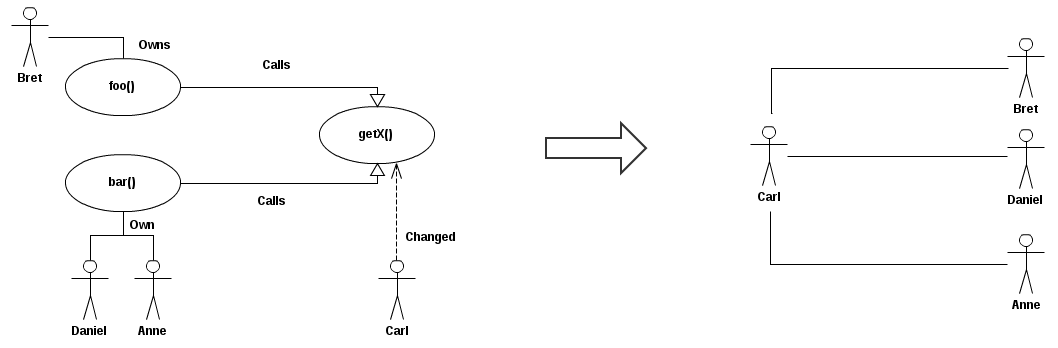
\includegraphics[width=0.9\textwidth]{images/TecNetwork}
\caption{A technical network for a changeset. Cody has changed method getX() which is being
called by Bart's method foo() as well as Daisy and Adam's method bar().\label{fig:network}}
\end{figure*}

\section{Methodology}

\subsection{Extracting Technical Networks}
% End goal
Our goal, is to create a technical network of contributors based on method ownership
and those method's call hierarchies effected by changesets. These networks will provide
dependency edges between contributors caused by changesets which may be 
identified as possible harmful pairings. (Figure~\ref{fig:network}). To achieve this goal,
we must identify contributor owners of methods, method call hierarchies (our technical
dependencies) and changeset effects on these hierarchies.

% Owners
To determine which contributors own which methods at a given changeset, we query
the Git repository. Git stores contributors of a file per line, which we can use to extrapolate
a percentage of ownership given a method inside the file.

% Call Graph
To extract method call hierarchies in a project at a given changeset, we must construct
a method call graph. Unlike other approaches such as Bodden's et al.~\cite{Bodden:2003:HVJ} 
of using byte code and whole projects, we built call graphs directly from source code files
inside of a changeset, 
which does not have the assumptions of being able to compile or have access to all project 
files. It is important, for us, to not require project compilation at each changeset because it is
an expensive operation as well as the changeset's effects may cause the project
to be unable to compile. Using source files also allows us to update our call graph
with changed files as opposed to completely rebuilding at 
every changeset. This creates a rolling call graph which 
can be used to show method hierarchy at each changeset inside a project opposed to
a static project view.

% Changeset effects
We now need to find a changeset's effect, if any, to the call hierarchy. We use the Git
software repository to determine what changes were made to any give file inside a 
changeset. Specifically, we look for methods modified by a changeset. We now use
the call graph to determine which methods call those that have been changed, which
gives the changeset's technical dependencies.

%Resulting network
These procedures, result in a technical network based on contributor method ownership 
inside a call hierarchy effected by a changeset (Figure~\ref{fig:network} left hand side).
We simplify the network by only using edges between contributors since we 
are only interested in discovering the problematic edges between contributors and not the 
methods themselves (Figure~\ref{fig:network} right hand side). This is our final technical 
network.

\subsection{Identifying Harmful Structures}
To identify harmful structures (edges) inside technical networks, we analyze 
edges in relation to discovered changeset failures. To determine whether a changeset 
was a success or failure (introduce a software failure), we use the approach of
Sliwerski et al.~\cite{Sliwerski:2005:CIF}. We then proceed in the following steps:

\begin{enumerate}
\item Identify all possible edges from the technical networks.
\item For each edge, count occurrences in technical networks of failed changesets.
\item For each edge, count occurrences in technical networks of successful changesets.
\item Determine if the edge is related to success or failure.
\end{enumerate}

To determine an edge's relation to success or failure, we create the value FI (failure
index) which represents the normalized chance of a changeset failure in the presence
of the edge. 

\begin{equation}
\text{FI} = \frac{ \text{edge}_{failed} / \text{total}_{failed}}{\text{edge}_{failed} / \text{total}_{failed} + \text{edge}_{success} / \text{total}_{success}}
\end{equation}

Contributor pairs with the highest FI value are said to be harmful structures
inside a project. We store these edges in Table~\ref{tab:ratio}. We also perform
a Fisher Exact Value test on edge appearance in successful and failed
changesets, and non-appearance in successful and failed changesets to only
consider statistically significant edges. 


\section{Results}
For this paper, we choose to study the Hibernate-ORM project which is an open source Java 
application hosted on GitHub\footnote{https://github.com/}. The issue tracking for this 
project is performed by Jira\footnote{http://www.atlassian.com/software/jira/overview}.

We chose this project because our tool only handles Java code and it is written in Java 
for all internal structures and control flow
and uses Git for version control. Hibernate-ORM also uses issue tracking software which 
is needed for determining changeset success or failure~\cite{Sliwerski:2005:CIF}.

In Hibernate-ORM, we found a total of X contributor pairs existed over the entire project, 
of which Y were found to be harmful inside of the system (A FI value of G or higher). 
We rank the pairings by their respective FI values(Table~\ref{tab:ratio}).

\begin{table}[h]
\begin{center}
\begin{tabular}{@{\hspace{.2cm}}ccc@{\hspace{.75cm}}c@{\hspace{.2cm}}c@{\hspace{.2cm}}}
\hline
Pair & Successful & Failed & FI & P-Value\\
\hline
(Daisy, Adam)	&	0&	14&	1.0000& 0.0001249		\\
(Cody, Bart)	&	1&	12&	0.9190& 0.003468	\\
(Emma, Fred)	&	1&	9&	0.8948& 0.02165      \\
\hline
\end{tabular}
\end{center}
\caption{The top 3 harmful contributor pairs found and ordered by FI.\label{tab:ratio}}
\end{table}

By recognizing known harmful pairings in new changeset networks, we can also predict that a
given changeset will fail based on these pairings FI value. We were able to predict 
W out of Z failures from a sample size of T  given changesets inside of Hibernate-ORM 
with Q false positives. More importantly, given 
the known harmful pairing, we can recommend communication between the two 
contributors.


\section{Conclusion and Future Work}
Technical dependencies are often used to predict software failures
in large software system~\cite{Pinzger:2008:DNP, Zimmermann:2008:PDU, Kim:2006:AIB}. 
We have found evidence that technical dependencies predict failures based on contributor
dependencies found in changesets. Through the contributor dependencies,
we can also give recommendations to contributors about whom to contact to
resolve potential issues.

In future work, we will add communication networks on a per commit basis as well. We plan
to investigate the congruence of these social and technical networks and its effects on 
software quality.



\bibliographystyle{IEEEtran}
\bibliography{paper}


% End of the paper
\end{document}
